\documentclass{article}
\setlength{\parindent}{0pt}
\setlength{\parskip}{2ex plus 0.5ex minus 0.2ex}
\usepackage[margin=1in]{geometry}
\usepackage{graphicx}
\usepackage{textcomp}
\usepackage{placeins}
\usepackage[T1]{fontenc}
\usepackage{gensymb}
\usepackage[utf8]{inputenc}
\usepackage{caption}
\usepackage[export]{adjustbox}
\graphicspath{{./figures/}}
% hyperref usually has to go last
\usepackage[hidelinks]{hyperref}
% but glossaries behaves best if after hyperref
\usepackage[acronym,toc]{glossaries}
%\newacronym{<++>}{<++>}{<++>}
\newacronym[longplural={metric tons of heavy metal}]{MTHM}{MTHM}{metric ton of heavy metal}
\newacronym{ABM}{ABM}{agent-based modeling}
\newacronym{AHTR}{AHTR}{Advanced High Temperature Reactor}
\newacronym{ANDRA}{ANDRA}{Agence Nationale pour la gestion des D\'echets RAdioactifs, the French National Agency for Radioactive Waste Management}
\newacronym{ANL}{ANL}{Argonne National Laboratory}
\newacronym{API}{API}{application programming interface}
\newacronym{ARE}{ARE}{Aircraft Reactor Experiment}
\newacronym{ARFC}{ARFC}{Advanced Reactors and Fuel Cycles}
\newacronym{ASME}{ASME}{American Society of Mechanical Engineers}
\newacronym{ATWS}{ATWS}{Anticipated Transient Without Scram}
\newacronym{BDBE}{BDBE}{Beyond Design Basis Event}
\newacronym{BIDS}{BIDS}{Berkeley Institute for Data Science}
\newacronym{CAFCA}{CAFCA}{ Code for Advanced Fuel Cycles Assessment }
\newacronym{CEA}{CEA}{Commissariat \`a l'\'Energie Atomique et aux \'Energies Alternatives}
\newacronym{CI}{CI}{continuous integration}
\newacronym{CNERG}{CNERG}{Computational Nuclear Engineering Research Group}
\newacronym{COSI}{COSI}{Commelini-Sicard}
\newacronym{COTS}{COTS}{commercial, off-the-shelf}
\newacronym{CSNF}{CSNF}{commercial spent nuclear fuel}
\newacronym{CTAH}{CTAHs}{Coiled Tube Air Heaters}
\newacronym{CUBIT}{CUBIT}{CUBIT Geometry and Mesh Generation Toolkit}
\newacronym{DAG}{DAG}{directed acyclic graph}
\newacronym{DANESS}{DANESS}{Dynamic Analysis of Nuclear Energy System Strategies}
\newacronym{DBE}{DBE}{Design Basis Event}
\newacronym{DESAE}{DESAE}{Dynamic Analysis of Nuclear Energy Systems Strategies}
\newacronym{DHS}{DHS}{Department of Homeland Security}
\newacronym{DOE}{DOE}{Department of Energy}
\newacronym{DRACS}{DRACS}{Direct Reactor Auxiliary Cooling System}
\newacronym{DRE}{DRE}{dynamic resource exchange}
\newacronym{DSNF}{DSNF}{DOE spent nuclear fuel}
\newacronym{DYMOND}{DYMOND}{Dynamic Model of Nuclear Development }
\newacronym{EBS}{EBS}{Engineered Barrier System}
\newacronym{EDZ}{EDZ}{Excavation Disturbed Zone}
\newacronym{EPA}{EPA}{Environmental Protection Agency}
\newacronym{EP}{EP}{Engineering Physics}
\newacronym{FCO}{FCO}{Fuel Cycle Options}
\newacronym{FCT}{FCT}{Fuel Cycle Technology}
\newacronym{FEHM}{FEHM}{Finite Element Heat and Mass Transfer}
\newacronym{FEPs}{FEPs}{Features, Events, and Processes}
\newacronym{FHR}{FHR}{Fluoride-Salt-Cooled High-Temperature Reactor}
\newacronym{FLiBe}{FLiBe}{Fluoride-Lithium-Beryllium}
\newacronym{GDSE}{GDSE}{Generic Disposal System Environment}
\newacronym{GDSM}{GDSM}{Generic Disposal System Model}
\newacronym{GENIUSv1}{GENIUSv1}{Global Evaluation of Nuclear Infrastructure Utilization Scenarios, Version 1}
\newacronym{GENIUSv2}{GENIUSv2}{Global Evaluation of Nuclear Infrastructure Utilization Scenarios, Version 2}
\newacronym{GENIUS}{GENIUS}{Global Evaluation of Nuclear Infrastructure Utilization Scenarios}
\newacronym{GPAM}{GPAM}{Generic Performance Assessment Model}
\newacronym{GRSAC}{GRSAC}{Graphite Reactor Severe Accident Code}
\newacronym{GUI}{GUI}{graphical user interface}
\newacronym{HLW}{HLW}{high level waste}
\newacronym{HPC}{HPC}{high-performance computing}
\newacronym{HTC}{HTC}{high-throughput computing}
\newacronym{HTGR}{HTGR}{High Temperature Gas-Cooled Reactor}
\newacronym{IAEA}{IAEA}{International Atomic Energy Agency}
\newacronym{INL}{INL}{Idaho National Laboratory}
\newacronym{JFNK}{JFNK}{Jacobian-Free Newton Krylov}
\newacronym{LANL}{LANL}{Los Alamos National Laboratory}
\newacronym{LBNL}{LBNL}{Lawrence Berkeley National Laboratory}
\newacronym{LCOE}{LCOE}{levelized cost of electricity}
\newacronym{LDRD}{LDRD}{laboratory directed research and development}
\newacronym{LFR}{LFR}{Lead-Cooled Fast Reactor}
\newacronym{LLNL}{LLNL}{Lawrence Livermore National Laboratory}
\newacronym{LMFBR}{LMFBR}{Liquid-Metal-cooled Fast Breeder Reactor}
\newacronym{LOFC}{LOFC}{Loss of Forced Cooling}
\newacronym{LOHS}{LOHS}{Loss of Heat Sink}
\newacronym{LOLA}{LOLA}{Loss of Large Area}
\newacronym{LP}{LP}{linear program}
\newacronym{MA}{MA}{minor actinide}
\newacronym{MCNP}{MCNP}{Monte Carlo N-Particle code}
\newacronym{MILP}{MILP}{mixed-integer linear program}
\newacronym{MIT}{MIT}{the Massachusetts Institute of Technology}
\newacronym{MOAB}{MOAB}{Mesh-Oriented datABase}
\newacronym{MOOSE}{MOOSE}{Multiphysics Object-Oriented Simulation Environment}
\newacronym{MOX}{MOX}{mixed oxide}
\newacronym{MSBR}{MSBR}{Molten Salt Breeder Reactor}
\newacronym{MSRE}{MSRE}{Molten Salt Reactor Experiment}
\newacronym{MSR}{MSR}{Molten Salt Reactor}
\newacronym{NAGRA}{NAGRA}{National Cooperative for the Disposal of Radioactive Waste}
\newacronym{NEAMS}{NEAMS}{Nuclear Engineering Advanced Modeling and Simulation}
\newacronym{NEUP}{NEUP}{Nuclear Energy University Programs}
\newacronym{NFCSim}{NFCSim}{Nuclear Fuel Cycle Simulator}
\newacronym{NGNP}{NGNP}{Next Generation Nuclear Plant}
\newacronym{NNSA}{NNSA}{National Nuclear Security Administration}
\newacronym{NQA1}{NQA-1}{Nuclear Quality Assurance - 1}
\newacronym{NRC}{NRC}{Nuclear Regulatory Commission}
\newacronym{NSF}{NSF}{National Science Foundation}
\newacronym{NSSC}{NSSC}{Nuclear Science and Security Consortium}
\newacronym{NUWASTE}{NUWASTE}{Nuclear Waste Assessment System for Technical Evaluation}
\newacronym{NWTRB}{NWTRB}{Nuclear Waste Technical Review Board}
\newacronym{OCRWM}{OCRWM}{Office of Civilian Radioactive Waste Management}
\newacronym{ORION}{ORION}{ORION}
\newacronym{ORNL}{ORNL}{Oak Ridge National Laboratory}
\newacronym{PARCS}{PARCS}{Purdue Advanced Reactor Core Simulator}
\newacronym{PBAHTR}{PB-AHTR}{Pebble Bed Advanced High Temperature Reactor}
\newacronym{PBFHR}{PB-FHR}{Pebble-Bed Fluoride-Salt-Cooled High-Temperature Reactor}
\newacronym{PEI}{PEI}{Peak Environmental Impact}
\newacronym{PH}{PRONGHORN}{PRONGHORN}
\newacronym{PRKE}{PRKE}{Point Reactor Kinetics Equations}
\newacronym{PSPG}{PSPG}{Pressure-Stabilizing/Petrov-Galerkin}
\newacronym{PWAR}{PWAR}{Pratt and Whitney Aircraft Reactor}
\newacronym{PyNE}{PyNE}{Python toolkit for Nuclear Engineering}
\newacronym{PyRK}{PyRK}{Python for Reactor Kinetics}
\newacronym{QA}{QA}{quality assurance}
\newacronym{RDD}{RD\&D}{Research Development and Demonstration}
\newacronym{RD}{R\&D}{Research and Development}
\newacronym{RELAP}{RELAP}{Reactor Excursion and Leak Analysis Program}
\newacronym{RIA}{RIA}{Reactivity Insertion Accident}
\newacronym{RIF}{RIF}{Region-Institution-Facility}
\newacronym{SFR}{SFR}{Sodium-Cooled Fast Reactor}
\newacronym{SINDAG}{SINDA{\textbackslash}G}{Systems Improved Numerical Differencing Analyzer $\backslash$ Gaski}
\newacronym{SKB}{SKB}{Svensk K\"{a}rnbr\"{a}nslehantering AB}
\newacronym{SNF}{SNF}{spent nuclear fuel}
\newacronym{SNL}{SNL}{Sandia National Laboratory}
\newacronym{STC}{STC}{specific temperature change}
\newacronym{SUPG}{SUPG}{Streamline-Upwind/Petrov-Galerkin}
\newacronym{SWF}{SWF}{Separations and Waste Forms}
\newacronym{SWU}{SWU}{Separative Work Unit}
\newacronym{TRISO}{TRISO}{Tristructural Isotropic}
\newacronym{TSM}{TSM}{Total System Model}
\newacronym{TSPA}{TSPA}{Total System Performance Assessment for the Yucca Mountain License Application}
\newacronym{ThOX}{ThOX}{thorium oxide}
\newacronym{UFD}{UFD}{Used Fuel Disposition}
\newacronym{UML}{UML}{Unified Modeling Language}
\newacronym{UOX}{UOX}{uranium oxide}
\newacronym{UQ}{UQ}{uncertainty quantification}
\newacronym{US}{US}{United States}
\newacronym{UW}{UW}{University of Wisconsin}
\newacronym{VISION}{VISION}{the Verifiable Fuel Cycle Simulation Model}
\newacronym{VV}{V\&V}{verification and validation}
\newacronym{WIPP}{WIPP}{Waste Isolation Pilot Plant}
\newacronym{YMR}{YMR}{Yucca Mountain Repository Site}

\makeglossaries
% cleveref only behaves if after hyperref & glossaries
\usepackage{cleveref}

\let\Oldsection\section
\renewcommand{\section}{\FloatBarrier\Oldsection}

\let\Oldsubsection\subsection
\renewcommand{\subsection}{\FloatBarrier\Oldsubsection}

\let\Oldsubsubsection\subsubsection
\renewcommand{\subsubsection}{\FloatBarrier\Oldsubsubsection}

\newcommand{\code}[1]{\texttt{#1}}

\title{Advanced Reactor Fuel Cycles Molten Salt Reactor Design}
\author{Alexander Lindsay, Andrei Rykhlevskii, Kathryn Huff} % As you author additions/changes, add
                                      % your name here!!!

% To do: Decide how to present figures in a way that they don't have both our
% figure labels as well as the original documents; also make sure we are
% reproducing those figures in an ethical way

\begin{document}
\maketitle

\section{Brief History}

The basis for this quick synopsis comes from \cite{wikipedia_molten_2016}.
Research into \glspl{MSR} began in earnest with the \gls{ARE}, with experiments
shared between \gls{ORNL} and what is now \gls{INL}. The \gls{ARE} used
NaF-ZrF$_4$-UF$_4$ (53-41-6 mol\%) as fuel. The reactor was moderated by
beryllium oxide (BeO), used liquid sodium as the secondary coolant, and had a
peak temperature around 860 \textdegree C. The \gls{ARE} managed to generate
100 MWh over the course of nine days in 1954. There was another reactor that
went critical at \gls{ORNL} in 1957 called the Pratt and Whitney Aircraft Reactor-1
(PWAR-1). Although it produced essentially no power, the PWAR-1 is still one of
only three critical MSRs ever built.

The most successful \gls{MSR}was the \gls{MSRE} which went
critical in 1965 and operated for four years at \gls{ORNL}. The \gls{MSRE} fuel was
LiF-BeF$_2$-ZrF$_4$-UF$_4$ (65-29-5-1 mol\%) with graphite core moderation. The
secondary coolant was 2LiF-BeF$_2$ (also known as FLiBe). Operating temperatures
went as high as 650 \textdegree C. \gls{MSRE} neutronics were meant to mimic that of
an epithermal thorium molten salt breeder reactor (MSBR); however, for the \gls{MSRE}
the expensive breeding blanket was sacrificed in favor of neutron
measurements. At full design power, the \gls{MSRE} operated at 7.4 MW$_{th}$. Over the
course of the late 1960s the \gls{MSRE} operated at full capacity for an equivalent of
1.5 years.

The logical follow-on from the \gls{MSRE} was the MSBR; however, the MSBR was never
constructed. Funding for the \gls{MSR}program was cut in favor of the
\gls{LMFBR} program. Consequently, as of today, the \gls{ARE},
PWAR-1, and \gls{MSRE} are the only critical MSRs ever operated.

\section{\gls{MSRE}}

\subsection{Salt properties}

\begin{figure}[htpb]
  \centering
  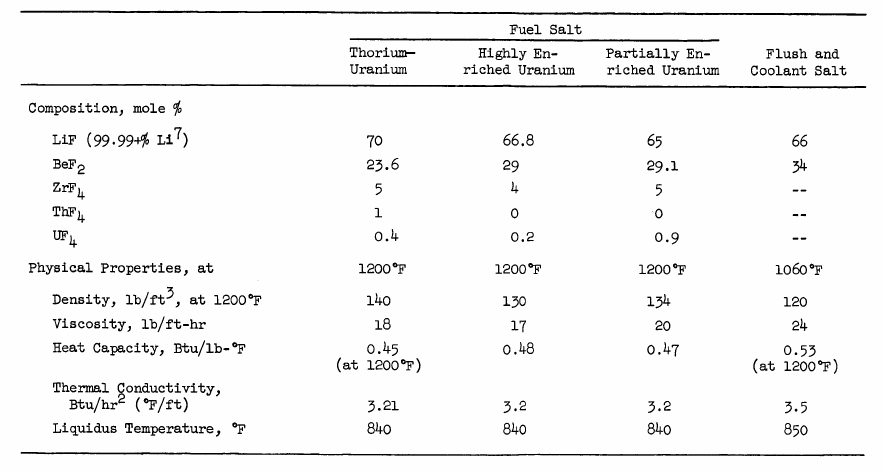
\includegraphics[max height=.5\textheight,max width=\textwidth,keepaspectratio]{salt_properties.png}
  \caption{Composition and properties of fuel, flush, and coolant
    salts \cite{robertson_msre_1965}.}
  \label{fig:salt_properties}
\end{figure}

The melting point of FLiBe is 459 \textdegree C and the boiling point is 1430
\textdegree C \cite{_flibe_2016}.

\subsection{Layout \& Equipment}

\begin{figure}[htpb]
  \centering
  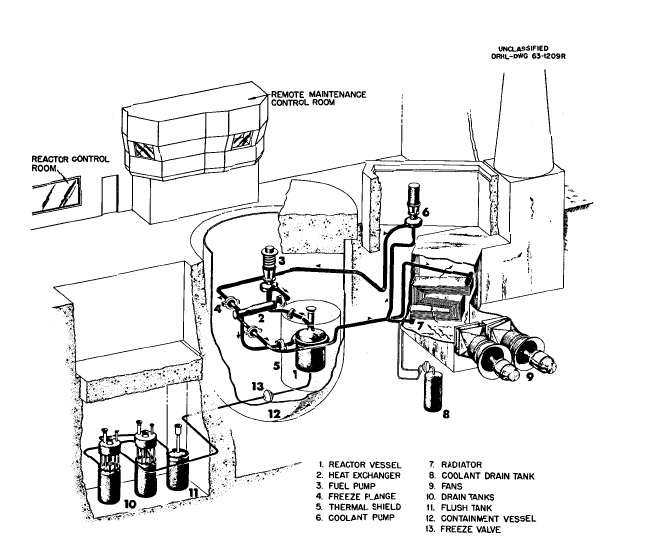
\includegraphics[max height=.5\textheight,max width=\textwidth,keepaspectratio]{flow_diagram.png}
  \caption{Macroscopic layout of the \gls{MSRE} \cite{robertson_msre_1965}}
  \label{fig:MSRE_layout}
\end{figure}

\subsubsection{Reactor vessel}
\label{sec:reactor}

A cutaway diagram of the \gls{MSRE} reactor is shown in
\cref{fig:MSRE_reactor}. Fuel enters through the inlet and is distributed evenly
along the outside of the reactor vessel in a small annular region of 1 inch
width \cite{robertson_msre_1965}. The fluid fuel then flows turbulently
downward, cooling the reactor vessel to within 5\textdegree F of the entering
bulk salt temperature (1175 \textdegree F) \cite{robertson_msre_1965}. This
down-flowing region is typically referred to as the \textit{downcomer}. The fuel
salt is collected in the lower plenum (lower \textit{space}) of the reactor
where straightening vanes remove the salt's rotational motion. The salt then
flows upward through approximately 1140 0.4-inch by 1.2-inch fuel channels that
are formed by machining grooves in the sides of the graphite moderator columns
\cite{robertson_msre_1965}; these are the regions where fission occurs.  The
graphite columns themselves have 2-inch by 2-inch square cross sections.
Nominal core volume is 90 ft$^3$, with 70 ft$^3$ occupied by graphite and 20
ft$^3$ occupied by fuel \cite{robertson_msre_1965}.  After flowing through the
core channels, the fuel collects in the upper plenum before exiting through the
outlet. At 10 MW, 0.6 MW of heat is generated in the graphite, 1.4 MW heat is
generated in the fuel outside the nominal core, and 8.0 MW is generated in the
fuel within the core \cite{robertson_msre_1965}. I'm very curious how those
numbers were determined.

\begin{figure}[htpb]
  \centering
  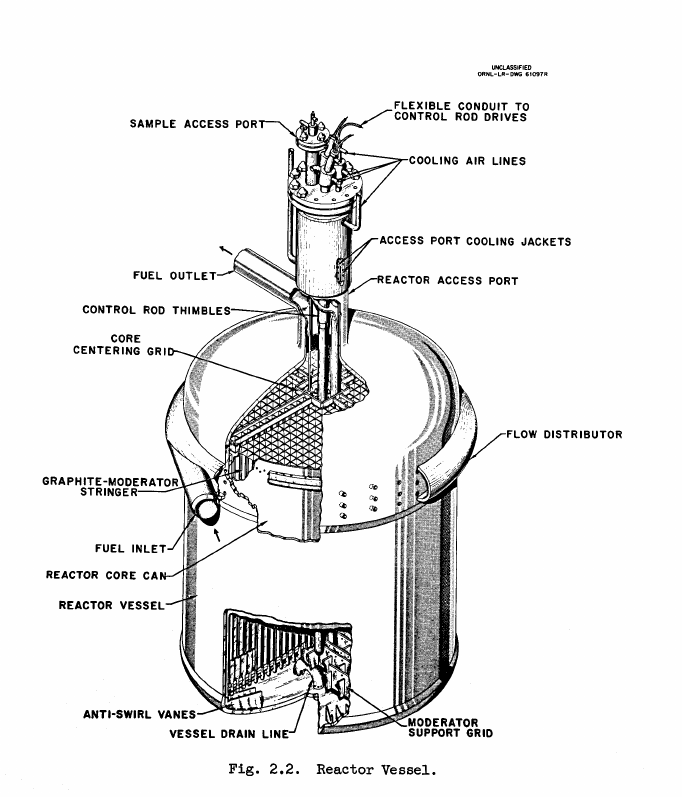
\includegraphics[max height=.5\textheight,max width=\textwidth,keepaspectratio]{MSRE_reactor_vessel.png}
  \caption{\gls{MSRE} reactor vessel \cite{robertson_msre_1965}.}
  \label{fig:MSRE_reactor}
\end{figure}

Flow in fuel channels is laminar; because both the graphite and fueld have good
thermal conductivities, the maximum temperature of the graphite is only about 60
\textdegree F above the mixed mean temperature of the adjacent fuel. Average and
maximum temperatures of graphite are 1255 \textdegree F and 1300 \textdegree F
respectively. The temperature of the fuel leaving the hottest channel in the
core is about 1260 \textdegree F. The fuel leaves the top of the reactor at 7
psig and an average temperature of 1225 \textdegree F \cite{robertson_msre_1965}.

Though studies were conducted with the \gls{MSRE} core surrounded by varying
thicknesses of reflector \cite{haubenreich_msre_1964}, the experimental design
was bare. This type of reactor design lends itself most naturally to a vacuum
boundary condition for neutrons (zero incoming flux) like that used in
\cite{dulla_neutron_2004}.

\subsubsection{Heat Exchanger}
\label{sec:heatx}

As mentioned in \cref{sec:reactor}, the fuel salt enters the reactor at 1175
\textdegree F and leaves at 1225 \textdegree F. In order to cool the fuel salt
back down to its reactor inlet temperature, the coolant salt flows through the
heat exchanger at 850 \gls{gpm} with inlet and outlet temperatures of 1025
\textdegree F and 1100 \textdegree F respectively \cite{robertson_msre_1965}.

\subsection{Reactivity considerations}

The \gls{MSRE} has a negative temperature coefficient of $6.4 - 9.9 \times10^{-5}$
($\Delta$k/k)/\textdegree F depending on the choice of
fuel \cite{robertson_msre_1965}. The \gls{MSRE}'s three control rods have a combined
worth of 5.6 - 7.6 \% $\Delta$k/k, again depending on the
fuel \cite{robertson_msre_1965}.

\begin{figure}[htpb]
  \centering
  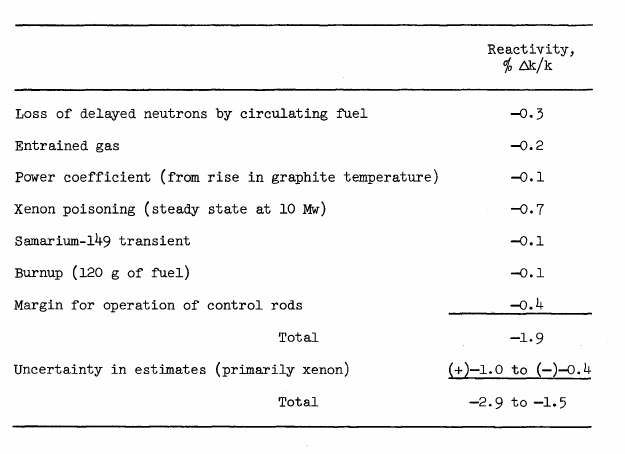
\includegraphics[max height=.5\textheight,max width=\textwidth,keepaspectratio]{reactivity-losses.png}
  \caption{Losses in reactivity associated with different
    phenomena \cite{robertson_msre_1965}.}
  \label{fig:reactivity_losses}
\end{figure}

\section{\gls{MSRE} adaption for modelling}

\subsection{Kophazi article review}

Kophazi developed a 3D time-dependent simulation that was validated against \gls{MSRE}
data \cite{kophazi_development_2009}. The model consists of a conventional
neutronics model extended to deal with the precursor drift that is unique to
MSRs and the core's thermal behavior. The thermal model includes the true
geometry of the fuel channels as well as the moderator connecting them. Salt
flow is assumed to be only in the reactor's axial direction, which reduces the
number of non-linear variables that have to be solved for.

\subsubsection{Neutronics}

Neutrons are described with time-dependent multi-group diffusion theory as shown
in \cref{eq:neutrons}:

\begin{equation}
\frac{1}{v_g}\frac{\partial \phi_g}{\partial t} - \nabla \cdot D_g \nabla \phi_g
+ \Sigma_g^r \phi_g = \sum_{g \ne g'}^G \Sigma_{g'\rightarrow g}^s \phi_{g'} + \chi_g^p \sum_{g' = 1}^G (1 - \beta)
\nu \Sigma_{g'}^f \phi_{g'} + \sum_i^I \lambda_i \chi_g^{d,i} C_i
\label{eq:neutrons}
\end{equation}

Delayed neutron precursors are described by \cref{eq:precursors}:

\begin{equation}
\frac{\partial C_i}{\partial t} = \sum_{g'= 1}^G \beta_i \nu \Sigma_{g'}^f
\phi_{g'} - \lambda_i C_i - \frac{\partial}{\partial z} u C_i
\label{eq:precursors}
\end{equation}

with the last term representing the effect of fuel advection. In
\cite{kophazi_development_2009}, \cref{eq:neutrons} is solved only in the
reactor core, whereas \cref{eq:precursors} is solved both in the core and in the
\gls{MSRE} external primary circuit. The external loop is modeled as a single pipe
with a volume equal to the total volume of all the external components and
pipelines of the primary circuitry \cite{kophazi_development_2009}. It is not
entirely clear how pipe cross sectional areas are handled, which would determine
the transit times of individual pieces of fluid and subsequently the
distribution of delayed neutron production in the external primary circuit. That
is a piece that would likely need to be included in detailed \gls{ARFC} accident
models.

As pointed out in \cite{kophazi_development_2009}, it is not possible to solve
\cref{eq:neutrons,eq:precursors} on the same mesh. \Cref{eq:neutrons} needs to
be solved over the entire reactor cross-section including fuel channels and the
graphite moderator in between, whereas \cref{eq:precursors} is only applicable
within the fuel channels. Kophazi solves this issue by introducing a fuel
fraction parameter, $p_f$, and creating effective fuel flow
channels. \Cref{fig:kophazi_homo} shows how Kophazi transforms the \gls{MSRE} unit
cell into neutronic and precursor elements. The number of effective fuel
channels in the unit cell is determined by the refinement of the neutron grid,
e.g. the \# of channels is equivalent to the number of neutronic elements in a
given \gls{MSRE} unit cell. Consequently, once the domain is discretized (Kophazi uses
the finite volume method), the delayed neutron source term (last term in
\cref{eq:neutrons}) is multiplied by the fuel fraction $p_f$. Homogenization of
the removal, scattering, and fission cross sections allows translation of the
model from the real to effective geometry. Details of the discretization can be
found in \cite{kophazi_development_2009}. Unfortunately, neither
\cite{kophazi_development_2009} or cited references for the DALTON code,
describe the boundary conditions used for neutrons.

\begin{figure}[htpb]
  \centering
  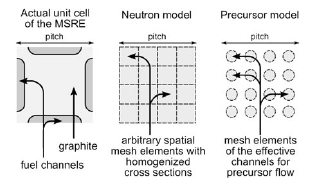
\includegraphics[max height=.5\textheight,max width=\textwidth,keepaspectratio]{kophazi_neutronics_discretization.png}
  \caption{Homogenized model of fuel channels \cite{kophazi_development_2009}}
  \label{fig:kophazi_homo}
\end{figure}

\subsubsection{Thermal Hydraulics}

Temperature in the fuel is determined by a 1-D convection model in the axial
direction. Moderator temperatures are calculated with a 3-D conduction
model. Coupling between the moderator and fuel temperatures is accomplished
through an axially varying heat transfer coefficient calculated with a Nusselt
correlation; see \cite{kophazi_development_2009} for details of the Nusselt
correlation. Thermal expansion of the fuel was not accounted for while
determining the reactor temperature profile; however, expansion is considered
($\kappa = 0.57 mg/cm^3 K$) when determining homogenized neutron
cross-sections. A model for the heat exchanger is included with a heat sink term
proportional to the temperature difference between fuel and coolant salts, with
the constant of proportionality determined from steady-state \gls{MSRE} operational
data. With the exception of the heat exchanger, the thermal code assumes zero
heat flux boundary conditions.

\subsubsection{Reactor Model}

Cell weighting and cross section homogenization calculations were carried out
using SCALE. In order to work with the 1D nature of the SCALE/CSAS/XSDRN code,
the actual \gls{MSRE} geometry was simplified as shown in \cref{fig:real-vs-model}
where the actual geometry is on the left and the model geometry is on the
right. Note that the far left sub-figure of \cref{fig:kophazi_homo} is the
zoomed, unit cell version of the left sub-figure of \cref{fig:real-vs-model}.

\begin{figure}[htpb]
  \centering
  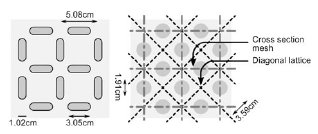
\includegraphics[max height=.5\textheight,max width=\textwidth,keepaspectratio]{kophazi-actual-vs-model-core-geometry.png}
  \caption{Left figure shows snapshot of actual \gls{MSRE} core geometry; to satisfy
    the 1D SCALE/CSAS/XSDRN code, the more regular geometry in the right figure
    is used \cite{kophazi_development_2009}}
  \label{fig:real-vs-model}
\end{figure}

Neutron cross sections were collapsed into eight energy groups, distributed
evenly on a logarithmic scale, with additional groups added in resonance and
thermal regions. Control rods were modeled with albedo boundary conditions for
thermal neutrons. More control rod modeling details can be found in
\cite{kophazi_development_2009}.

Neutron and thermal calculations are performed on separate grids. The axial and
horizontal neutron grids are both shown in \cref{fig:neutron-grid}. It includes
regions for the lower and upper salt plena, downcomer, and three control rods. A
section of the horizontal thermal grid is shown in \cref{fig:thermal-grid}. In
general, the thermal grid is finer than the neutron grid. Thermal and neutronic
calculations are coupled in the following way. Each cell of the neutronics mesh
(containing both fuel and moderator, recall \cref{fig:kophazi_homo}) is
considered to have uniform cross-sections. To generate these constant
cross-sections in each neutronic cell, the fine-mesh temperature fields from
the thermal calculation (called THERM) are spatially averaged using an auxiliary
program. This averaged neutron-cell-specific temperature is then used in
conjunction with cross section interpolation tables generated by SCALE to
determine the macroscopic cross sections for each neutron cell in the
simulation.

\begin{figure}[htpb]
  \centering
  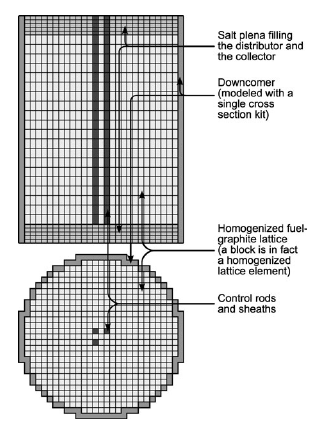
\includegraphics[max height=.5\textheight,max width=\textwidth,keepaspectratio]{3d-neutron-grid.png}
  \caption{Grid for cross section homogenization and neutron cross sections
    \cite{kophazi_development_2009}}
  \label{fig:neutron-grid}
\end{figure}

\begin{figure}[htpb]
  \centering
  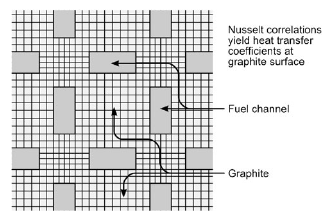
\includegraphics[max height=.5\textheight,max width=\textwidth,keepaspectratio]{cross-section-of-thermal-grid.png}
  \caption{Cross-section of thermal grid \cite{kophazi_development_2009}}
  \label{fig:thermal-grid}
\end{figure}

Feedback from the neutron to thermal calculations is accomplished by translating
the power distribution from the coarse neutron grid to the fine thermal grid
using another auxiliary program. This power distribution is then used as a heat
source in the thermal code.

\subsection{\gls{ARFC} \gls{MSRE} Model Design Plan}

\begin{enumerate}
\item Test whether \code{gmsh} can generate heterogeneous 3D mesh structure
  like that in the actual \gls{MSRE} geometry.
\item For expected range of temperatures and some defined sequence of
  temperature step sizes, generate table of few-group neutronics cross sections
  with \code{SERPENT}.
  \begin{itemize}
    \item If \code{gmsh}, or that failing \code{cubit}, is capable of generating
      heterogeneous grid, we can generate unique cross regions for each region
    \item If we cannot generate heterogeneous grid, we will have to homogenize
      the cross sections similar to what is done in
      \cite{kophazi_development_2009}.
  \end{itemize}
\item Armed with tables for quick interpolation of cross sections, we should be
  able to perform coupled calculations for neutron density and
  temperature.
  \begin{itemize}
    \item As a first pass, the fuel salt flow velocity can be a user input as
            opposed to a non-linear variable that is a function of temperature.
    \item However, the natural convection impacts on salt flow will
            significantly contribute to reactor dynamics and the ultimate goal
            will be to couple neutron flux and flow directly via
            temperature.
    \item We will need to decide whether neutron and temperature calculations
      should be performed on the same grid, and in transient calculations
      whether those two fields should be updated on the same step-size.
      \begin{itemize}
        \item If not using the same grid and/or step-size, the neutronic and
          temperature calculations will need to be split into their own
          applications and coupling will have to be performed using the MOOSE
          multi-app system.
      \end{itemize}
  \end{itemize}
\end{enumerate}

\section{MSBR}

The most detailed report on \gls{ORNL}'s molten salt breeder reactor is the technical
report by Robertson \cite{robertson_conceptual_1971}. A nice overview of the
MSBR geometry is shown in \cref{fig:vertical,fig:horizontal,fig:zoom_horiz}.

\begin{figure}[htpb]
  \centering
  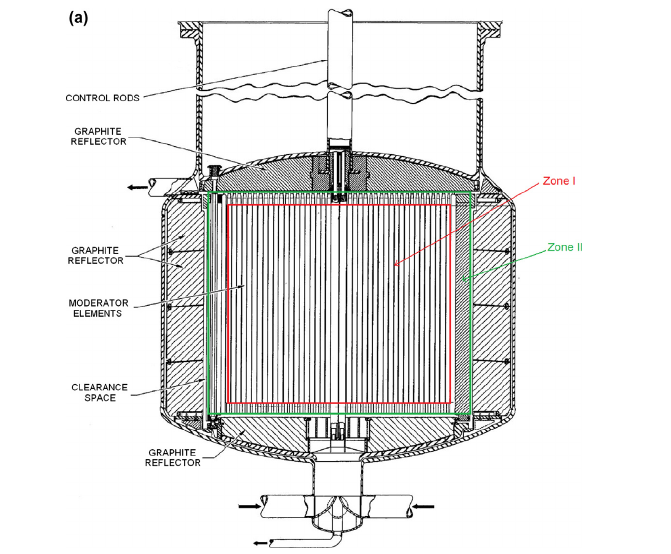
\includegraphics[max height=.5\textheight,max width=\textwidth,keepaspectratio]{vertical_MSBR_cross_section.png}
  \caption{Vertical cross section of MSBR.}
  \label{fig:vertical}
\end{figure}
\begin{figure}[htpb]
  \centering
  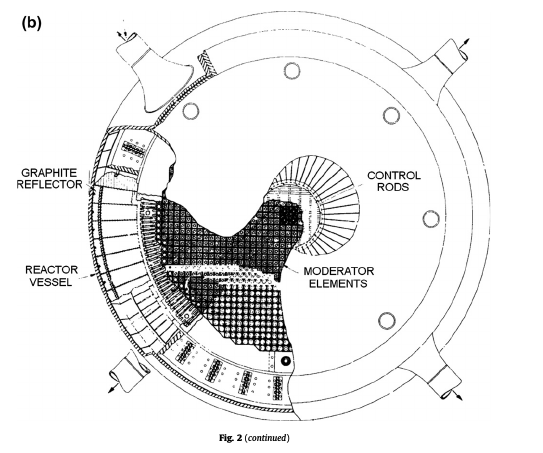
\includegraphics[max height=.5\textheight,max width=\textwidth,keepaspectratio]{horizontal_MSBR_cross_section.png}
  \caption{Horizontal cross section of MSBR.}
  \label{fig:horizontal}
\end{figure}
\begin{figure}[htpb]
  \centering
  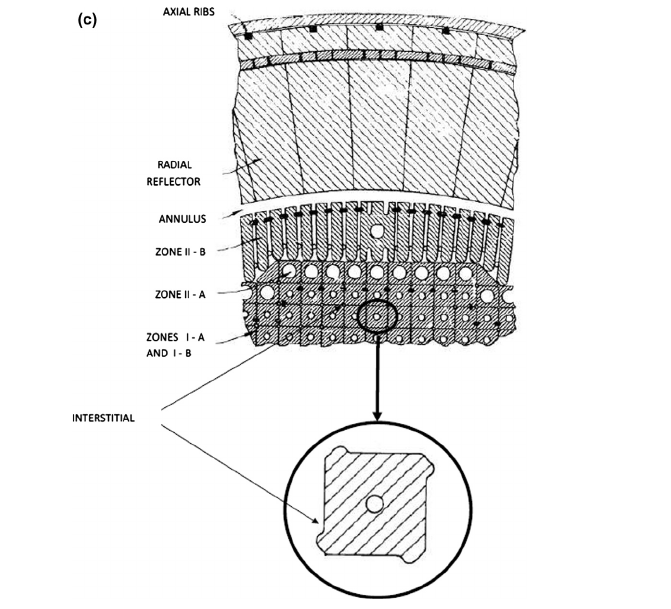
\includegraphics[max height=.5\textheight,max width=\textwidth,keepaspectratio]{zoomed_horizontal_MSBR_cross_section.png}
  \caption{Zoomed in horizontal cross-section of MSBR. Shows presence of
    interstitials between graphite block elements in zone 1 of the reactor.}
  \label{fig:zoom_horiz}
\end{figure}

\section{Simplified models}

\subsection{MSBR children}

\subsubsection{Cammi et. al.}

This model is based on the multi-physics model by
\cite{cammi_multi-physics_2011}.

Model's simplifications:
\begin{enumerate}
	\item Considered only one channel (diameter ~0.05 m)
	\item Hollow cylinder instead of block with a hole (with keeping the same fuel to graphite ratio)
	\item Infinite length of the channel (z tends to infinity)
\end{enumerate}

\begin{figure}[htpb]
  \centering
  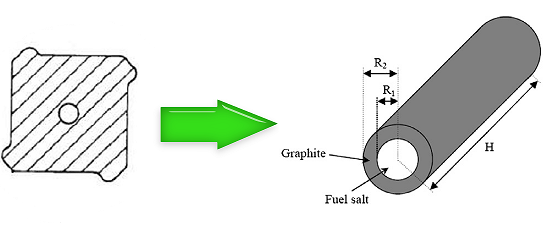
\includegraphics[max height=.5\textheight,max width=\textwidth,keepaspectratio]{Cammi_simplification_1.png}
  \caption{Cammi's simplification of MSBR's geometry
        \cite{cammi_multi-physics_2011}.}
  \label{fig:simlification}
\end{figure}

Neutronics Boundary Conditions.
\begin{enumerate}
	\item \textit{Inlet boundary}. The "vacuum" condition is adopted for the fast and thermal neutron fluxes. The circulation of delayed neutron precursors is taken into account considering that a certain amount of DNPs can return into the core from the external loop:

	\[ C_{i,in}(t) = C_{i,out}(t- \tau_{EL})\exp(- \lambda_i \tau_{EL}) \]
	\item \textit{Outlet boundary}. "Vacuum" condition for fast and thermal neutrons.
	\item \textit{Wall and central boundaries.} Symmetry boundary conditions are imposed for the neutron fluxes at r=0 and $ r=R_2 $.
\end{enumerate}

Flow and heat transfer boundary conditions.
\begin{enumerate}
	\item \textit{Inlet boundary}. The inlet velocity is given as $u_z = U_{in}=1.47 m/s$ and $u_r=0$. Turbulent kinetic energy $k_{in}=0.007 m^2/s^2$. Turbulent dissipation rate $\epsilon_{in}=0.033 m^2/s^2 $. $T_F=T_in=839K$.
	\item \textit{Outlet boundary}. The "local one-way method" is exploited for u,k,$\epsilon$, and $T_F$.
	\item \textit{Central boundaries.} Symmetry conditions are considered on the axis of the channel.
	\item \textit{Wall and central boundaries.} "Wall function approach" that use empirically-based relations in turbulent flows near solid boundaries in order to describe the velocity and temperature profile in the thin boundary layer near the wall, instead of solving the turbulence equations.
\end{enumerate}

\begin{figure}[htpb]
  \centering
  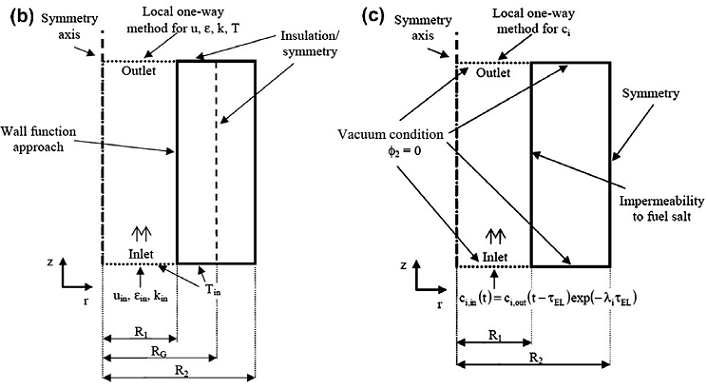
\includegraphics[max height=.5\textheight,max width=\textwidth,keepaspectratio]{Cammi_simplification_2.png}
  \caption{(b) Fluid flow and heat transfer boundary conditions; (c) neutron
        flux and DNP boundary conditions \cite{cammi_multi-physics_2011}.}
  \label{fig:simlification-2}
\end{figure}

\FloatBarrier
\clearpage
\printglossary[type=\acronymtype]
\bibliographystyle{unsrt}
\bibliography{MSR-design}
\end{document}
